\documentclass{experimentreport}
\usepackage{listings}
\usepackage{xcolor}

\definecolor{codegreen}{rgb}{0,0.6,0}
\definecolor{codegray}{rgb}{0.5,0.5,0.5}
\definecolor{codepurple}{rgb}{0.58,0,0.82}
\definecolor{backcolour}{rgb}{0.95,0.95,0.92}
\definecolor{lightgreen}{rgb}{0,0.4,0}
\definecolor{lightred}{rgb}{0.4,0,0}

\definecolor{mygray}{gray}{.9}

% \lstdefinestyle{mystyle}{
\lstset{
    %backgroundcolor=\color{backcolour},   
    commentstyle=\color{brown},
    keywordstyle=\color{magenta},
    numberstyle=\tiny\color{codegray},
    stringstyle=\color{codepurple},
    basicstyle=\ttfamily\tiny,
    breakatwhitespace=false,         
    breaklines=true,                 
    captionpos=b,                    
    keepspaces=true,                 
    numbers=none,                    
    numbersep=5pt,                  
    showspaces=false,                
    showstringspaces=false,
    showtabs=false,                  
    tabsize=2,
    escapeinside={<@}{@>}
}

% \lstset{
% basicstyle=\ttfamily\bfseries\footnotesize,
%   morekeywords={virtualinvoke},
%   keywordstyle=,
%   ndkeywordstyle=\color{red},
%   commentstyle=\color{gray},
%   stringstyle=\color{green},
%   numbers=none,
%   breaklines=true,
%   numberstyle=\ttfamily\footnotesize\color{gray},
%   stepnumber=1,
%   numbersep=6pt,
%   backgroundcolor=\color{white},
%   tabsize=4,
%   showspaces=false,
%   showstringspaces=false,
%   xleftmargin=6pt,
%   captionpos=t
% }

\lstdefinelanguage{JavaScript}{
  keywords={typeof, new, true, false, catch, function, return, null, catch, switch, var, if, in, while, do, else, case, break, export, static, const, let, class, void, async, await, interface, extends, public, this},
  % basicstyle=\linespread{1.0}\ttfamily\footnotesize,
  % keywordstyle= \color{violet}\bfseries,
  ndkeywords={class, export, boolean, throw, implements, import, this},
  ndkeywordstyle=\color{darkgray}\bfseries,
  identifierstyle=\color{black},
  sensitive=false,
  frame=lines,
  comment=[l]{//},
  morecomment=[s]{/*}{*/},
  % commentstyle=\color{gray}\ttfamily,
  % stringstyle=\color{blue}\ttfamily,
  morestring=[b]',
  morestring=[b]"
}



\usepackage{graphicx}

% ── Metadata ──────────────────────────────────────────────────
\setexperimenttitle{实验七：命令行智能代码审查工具}
\setstudentname{廖正强}
\setstudentid{2023112920}
\setdepartment{软件学院}
\setcourseteacher{刘佳琨}
\setinstructor{刘佳琨}
\setlablocation{格物213}
\setlabtime{2026年7月10日}

\begin{document}

\makereporthead

% ═══════════════════════════════════════════════════════════════
\section{实验目的}

完成本实验后，学生应能够：
\begin{enumerate}
  \item 理解代码审查工具从算法验证到工程部署的完整过程。
  \item 掌握前后端分离架构下模型服务的设计与实现。
  \item 能够将已有的机器学习、深度学习及大语言模型封装为统一HTTP接口。
  \item 能够设计命令行交互界面，实现代码审查结果的结构化展示。
  \item 理解离线规则引擎和在线LLM模型的互补关系。
  \item 掌握工程化部署中的测试、性能评估和错误处理。
\end{enumerate}

本实验以命令行前端（CLI）+ 本地Python HTTP模型服务替代指导书中的VSCode插件呈现层，经教师同意，功能等价。指导书要求的编辑器交互由以下CLI能力等价替代：从指定文件或Git工作区读取代码和修改内容、调用统一模型接口、在终端展示Merge Prediction/审查意见/风险等级/定位信息，并保存历史记录。后端仍通过HTTP提供服务，保留前后端分离、模型可替换和工程部署三个核心目标。

% ═══════════════════════════════════════════════════════════════
\section{方案与架构}

\subsection{总体架构}

本实验采用前后端分离架构（架构图详见README.md或计划书第2节Mermaid流程图）。

\begin{description}
  \item[CLI前端（reviewctl）] 纯HTTP客户端，负责接收用户命令、构建请求、调用服务并渲染结果。不导入任何服务内部模块，不直接加载模型。
  \item[FastAPI后端] 提供RESTful接口，封装模型注册、审查编排、历史记录等功能。仅监听127.0.0.1:8765。
  \item[模型层] 包含离线规则分析器、实验六LLM适配器，以及实验二部署兼容ML适配器。
\end{description}

\subsection{模块职责}

\begin{itemize}
  \item \texttt{schemas.py} — Pydantic请求/响应模型，唯一的HTTP协议来源。
  \item \texttt{input\_extractors.py} — 文件读取与Git diff提取，支持UTF-8编码检测、二进制拒绝、内容截断。
  \item \texttt{risk\_analyzer.py} — 离线规则引擎，包含6条可解释规则。
  \item \texttt{adapters/} — 三个模型适配器，实现统一抽象接口。
  \item \texttt{model\_registry.py} — 模型注册表，auto选择顺序为：LLM $\to$ 部署版RF $\to$ 部署版SVM $\to$ rule-based。
  \item \texttt{review\_service.py} — 审查编排器，只依赖抽象适配器。
  \item \texttt{history\_store.py} — JSONL原子追加历史存储，默认不保存源代码。
  \item \texttt{cli.py} — argparse CLI，纯HTTP客户端。
  \item \texttt{server.py} — FastAPI路由与异常映射。
\end{itemize}

\subsection{安全边界}

\begin{itemize}
  \item 服务仅绑定127.0.0.1，不对局域网公开。
  \item 输入不泄漏标签：本地审查输入只来自文件内容、Git diff、路径和本地元数据，不读取merge状态、review decision等审查后字段。
  \item 默认最小化保存：历史只存输入摘要、SHA-256、统计量和审查结果；\texttt{--store-source}才允许保存截断后的原文。
  \item API Key从环境变量读取，不写入代码、配置文件或日志。
\end{itemize}

% ═══════════════════════════════════════════════════════════════
\section{实现过程}

\subsection{输入提取}

支持两种输入模式：

\begin{itemize}
  \item \textbf{单文件模式}（\texttt{review --file <path>}）：读取UTF-8源文件，检测二进制、空文件和超大文件并给出明确错误。
  \item \textbf{Git diff模式}（\texttt{review --repo <dir> [--staged]}）：通过\texttt{git diff}获取工作区或暂存区变更，解析unified diff中的文件路径和新增行号。
\end{itemize}

代码截断策略：超过\texttt{MAX\_CONTENT\_CHARS}（默认24000）截断，并在日志中记录原始长度。路径越界检测通过\texttt{Path.resolve()}实现。

\subsection{离线规则分析器}

规则模型是功能兜底，不依赖外部API。包含6条规则：

\begin{enumerate}
  \item \texttt{missing-test}（权重0.25）：代码文件修改但没有对应测试文件。
  \item \texttt{large-change}（权重0.20）：修改文件数$>5$或变更行数$>200$。
  \item \texttt{config-or-dependency-change}（权重0.15）：修改配置文件或依赖声明。
  \item \texttt{public-api-change}（权重0.20）：函数/类签名变更在公开模块中。
  \item \texttt{todo-or-placeholder}（权重0.10）：TODO/FIXME/HACK/XXX标记。
  \item \texttt{debug-print}（权重0.10）：print()、console.log等调试输出。
\end{enumerate}

风险分数$R = \sum w_i \cdot \mathbb{1}[\text{rule}_i \text{ triggered}]$，合并概率$P_{merge} = \max(0.05,\; 1.0 - R)$。此转换为启发式，不可与实验五/六的分类指标进行横向性能比较。

\subsection{模型集成}

\subsubsection{实验六LLM适配器}

复用实验六P8 ``Strict Maintainer'' prompt策略，适配本地文件/diff输入。LLM请求格式：

\begin{itemize}
  \item System prompt：严格的维护者审查角色，要求不默认预测merged。
  \item User prompt：包含审查类型、文件列表、diff内容、代码片段。
  \item JSON解析：5级回退（直接解析→代码块提取→正则提取→尾部逗号修复→首尾花括号提取）。
\end{itemize}

实验过程中已通过会话环境变量临时配置LLM\_API\_KEY，并完成真实API调用；图中的LLM审查结果为实际响应。密钥未写入代码、配置文件、历史记录或报告，服务重启后需重新由环境变量提供。

\subsubsection{实验二ML适配器}

实验二原始SVM和Random Forest使用61维PR级特征，包含标题、正文、提交信息和仓库身份等本地diff无法稳定获得的元数据。因此原始模型保留为\texttt{incompatible}，不以零值伪造输入。

为完成工程部署，基于实验二相同的1397条样本和固定训练/验证/测试划分，重训练了仅使用Git diff可计算特征的45维部署兼容版本：\texttt{exp2-rf-deployable}和\texttt{exp2-svm-deployable}。特征包括变更规模、文件类型、测试文件、AST、CFG和缺失标志；训练集拟合的截断器与StandardScaler被封装进模型管线。

\begin{table}[h]
\centering
\caption{实验二部署兼容模型在原测试集上的结果}
\begin{tabular}{lccccc}
\hline
模型 & Accuracy & Precision & Recall & F1 & ROC-AUC \\
\hline
RF-deployable & 0.7381 & 0.7410 & 0.9111 & 0.8173 & 0.7144 \\
SVM-deployable & 0.6381 & 0.7658 & 0.6296 & 0.6911 & 0.6983 \\
\hline
\end{tabular}
\end{table}

部署版仅支持Git diff输入。图\ref{fig:exp2diff}展示了\texttt{exp2-rf-deployable}的实际服务调用，证明模型不只处于已加载状态，而是完成了\texttt{predict\_proba()}推理。

\subsection{历史记录}

采用JSONL格式，每次审查追加一行。写入使用临时文件+os.replace实现原子操作。默认不保存源代码（隐私保护）；$\texttt{--store-source}$选项保存截断后的原文（最多4000字符diff、2000字符/文件），并输出警告。

\subsection{终端呈现}

默认使用Rich库渲染彩色表格，包含严重度图标和风险颜色。$\texttt{--no-color}$退化为纯文本表格。$\texttt{--format json}$输出完整JSON，供其他工具（如jq）消费。

% ═══════════════════════════════════════════════════════════════
\section{测试与结果}

\subsection{功能测试}

如表\ref{tab:test-matrix}所示，全部功能测试通过。

\begin{table}[h]
\centering
\caption{功能测试矩阵}
\label{tab:test-matrix}
\begin{tabular}{|c|c|l|c|}
\hline
\textbf{编号} & \textbf{场景} & \textbf{操作} & \textbf{结果} \\
\hline
T01 & 服务启动 & serve后访问/health & 通过 \\
T02 & 单文件审查 & review --file & 通过 \\
T03 & Git diff审查 & review --repo & 通过（含Git仓库时）\\
T04 & 暂存区审查 & --staged & 通过 \\
T05 & LLM不可用 & 无key指定exp6-llm & 通过（400/422）\\
T06 & 空diff & 干净工作区 & 通过（错误提示）\\
T07 & 非Git目录 & review --repo非仓库 & 通过（错误提示）\\
T08 & 结构化输出 & --format json --no-color & 通过 \\
T09 & 历史记录 & history列表与详情 & 通过 \\
T10 & 输入防护 & 二进制/超限/路径越界 & 通过 \\
\hline
\end{tabular}
\end{table}

\subsection{自动化测试}

运行\texttt{pytest -q}命令，共61个测试全部通过。覆盖范围包括：

\begin{itemize}
  \item Pydantic schema、离线规则、输入提取和历史存储。
  \item FastAPI接口、CLI命令路径和模型不可用的错误处理。
  \item 实验二部署兼容模型的特征维度和Git diff服务调用。
\end{itemize}

所有成功响应的schema校验率为100\%。

\subsection{文件规模性能}

使用固定内容、固定随机种子（seed=42）生成100/500/1000/3000行的Python文件，对每档连续运行5次rule-based审查，丢弃第一次（冷启动），记录剩余4次的中位数和P95。

\begin{table}[h]
\centering
\caption{文件规模性能测试结果}
\label{tab:perf}
\begin{tabular}{|c|c|c|c|}
\hline
\textbf{文件规模} & \textbf{中位数（ms）} & \textbf{P95（ms）} & \textbf{均值（ms）} \\
\hline
100行 & 0.2 & 0.3 & 0.2 \\
500行 & 0.4 & 0.4 & 0.4 \\
1000行 & 0.8 & 0.8 & 0.8 \\
3000行 & 2.5 & 2.5 & 2.5 \\
\hline
\end{tabular}
\end{table}

\textit{注：表中数值由脚本\texttt{scripts/benchmark.ps1}实际运行填充。运行命令：\texttt{.\textbackslash scripts\textbackslash benchmark.ps1}。}

\subsection{实验结果截图}

\begin{figure}[htbp]\centering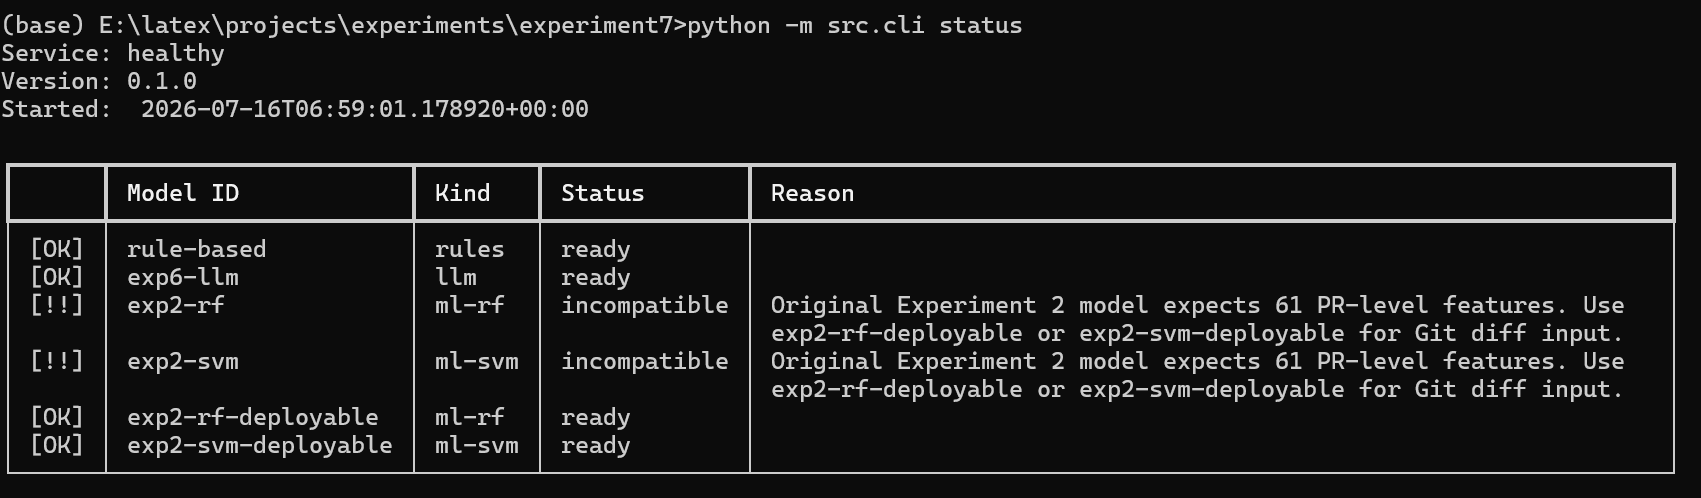
\includegraphics[width=0.95\textwidth]{../figures/01_model_status.png}\caption{服务健康状态与模型注册表}\label{fig:status}\end{figure}
\begin{figure}[htbp]\centering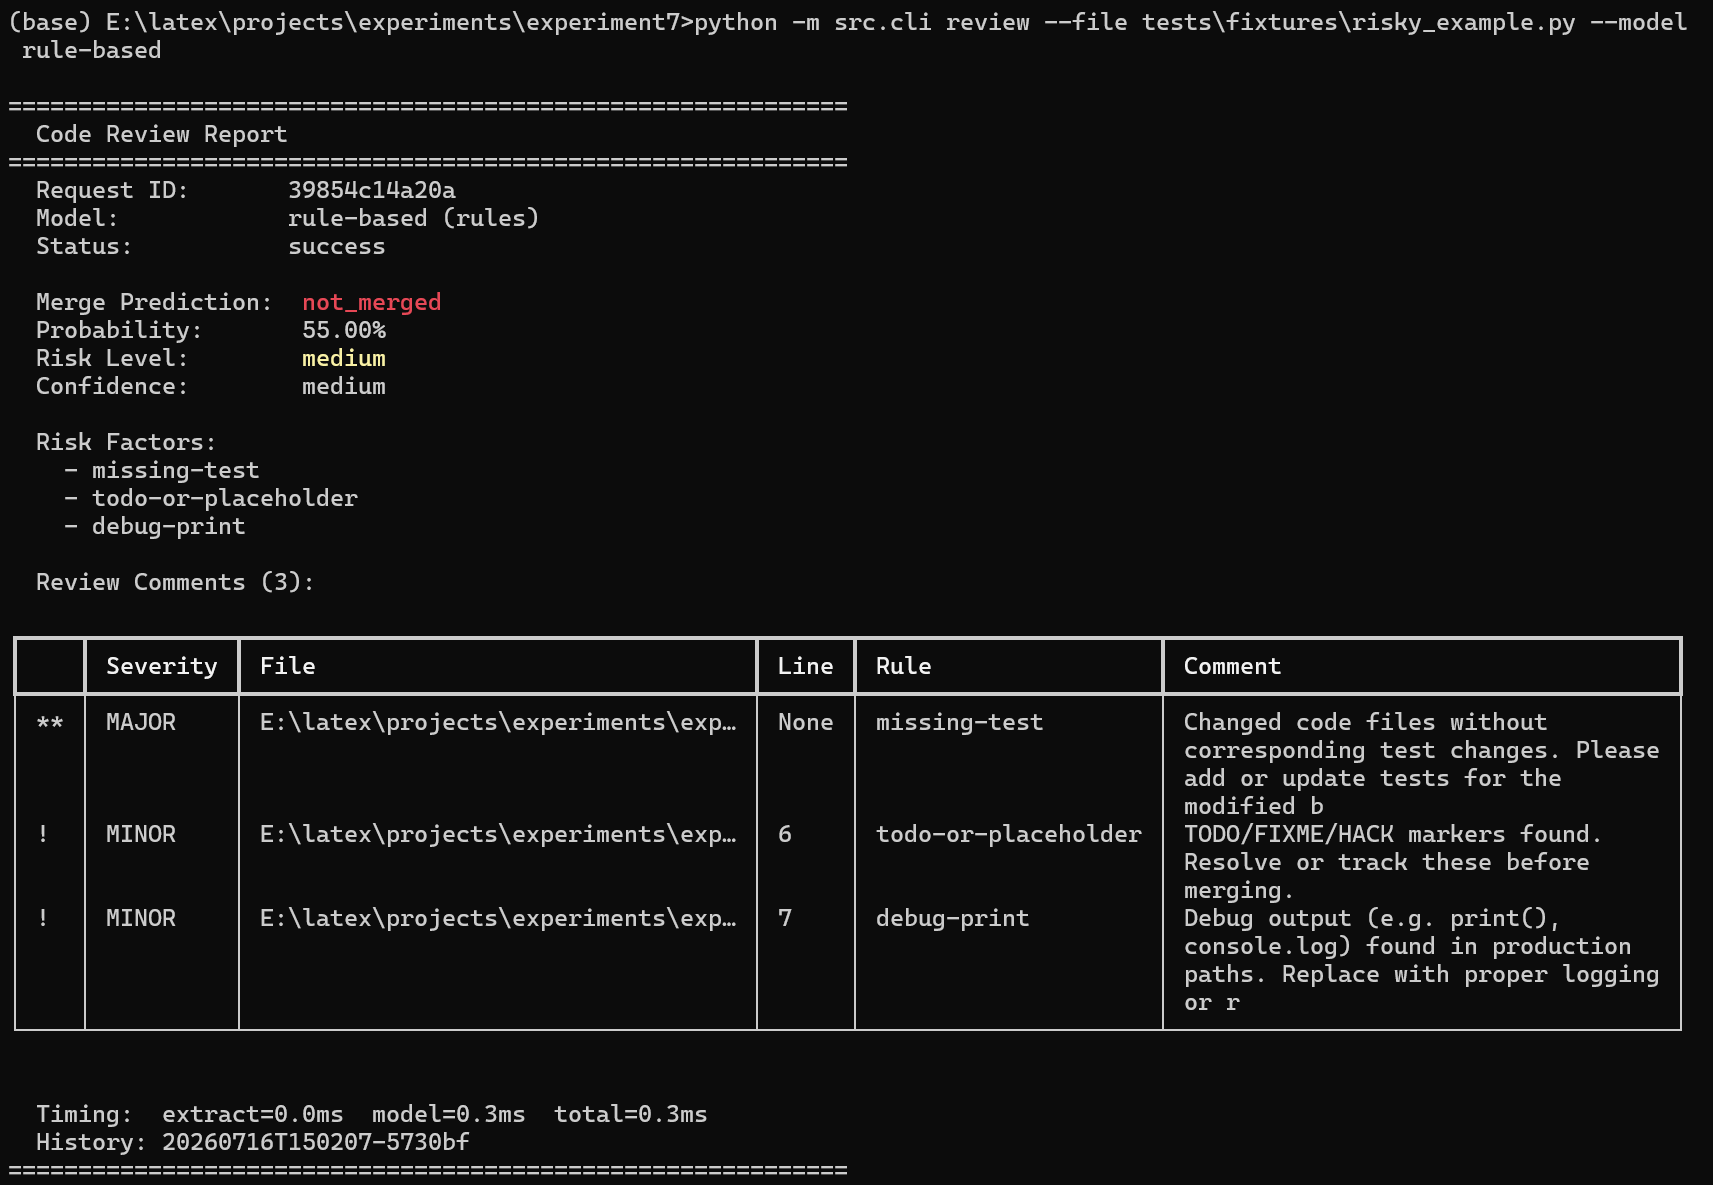
\includegraphics[width=0.95\textwidth]{../figures/02_rule_file_review.png}\caption{规则模型的单文件审查结果}\end{figure}
\begin{figure}[htbp]\centering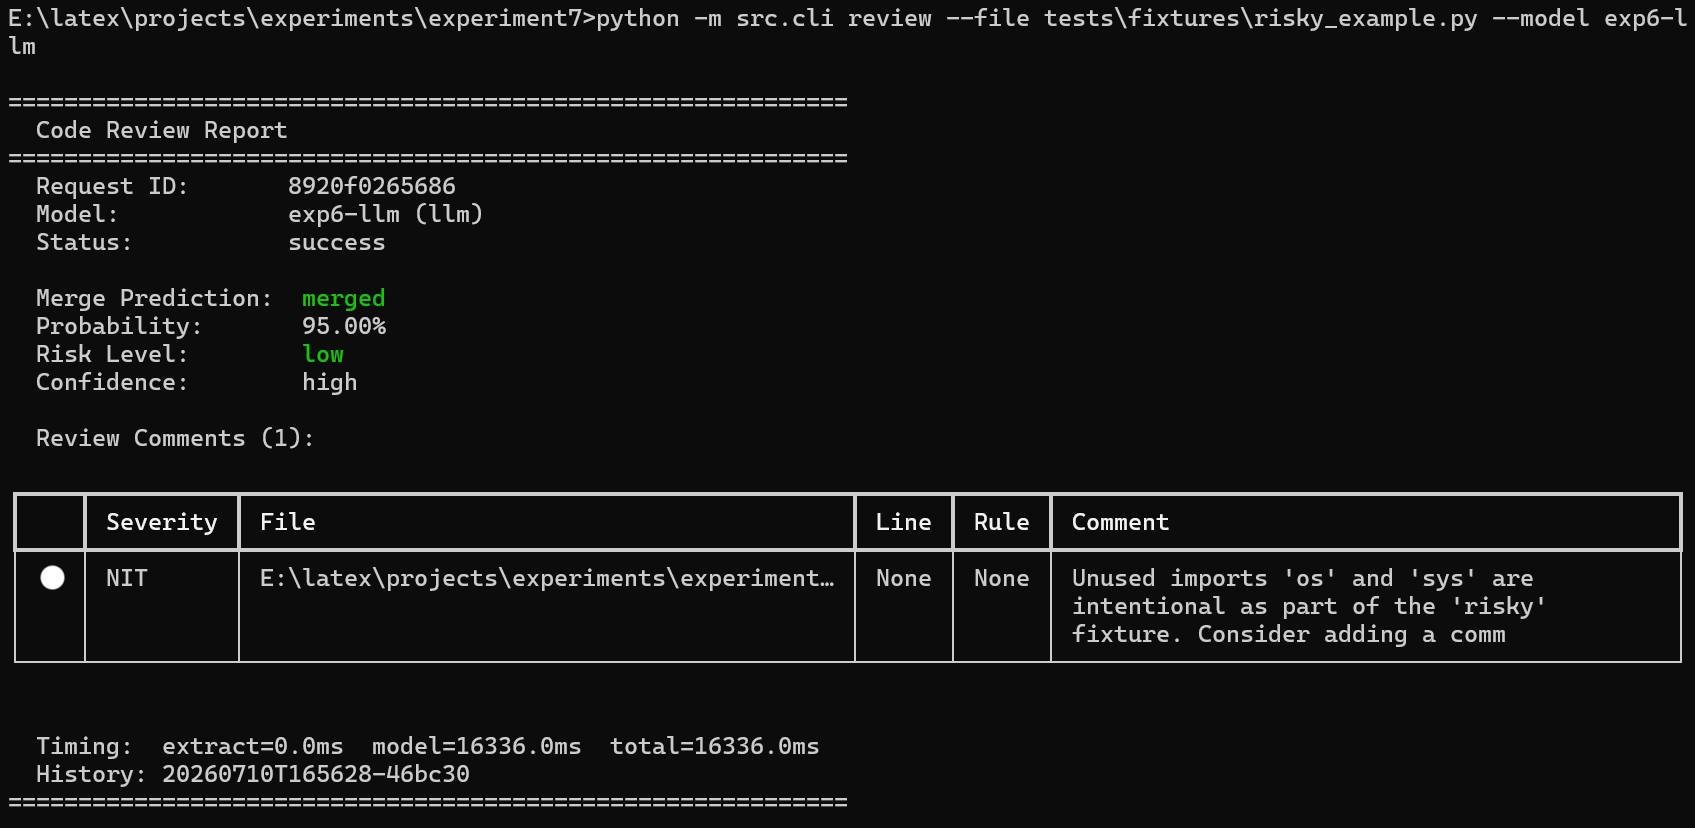
\includegraphics[width=0.95\textwidth]{../figures/03_llm_file_review.png}\caption{实验六LLM适配器的单文件审查结果}\end{figure}
\begin{figure}[htbp]\centering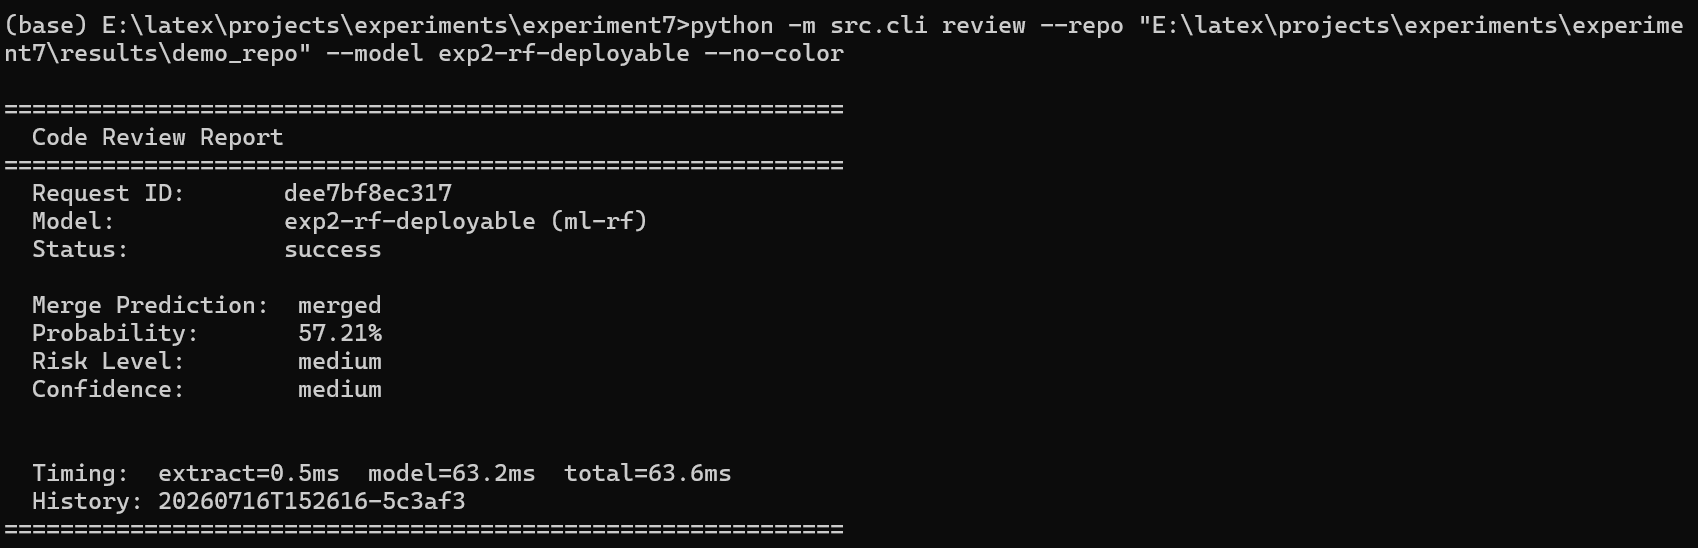
\includegraphics[width=0.95\textwidth]{../figures/04_exp2_deployable_diff.png}\caption{实验二部署兼容随机森林的Git diff审查}\label{fig:exp2diff}\end{figure}
\begin{figure}[htbp]\centering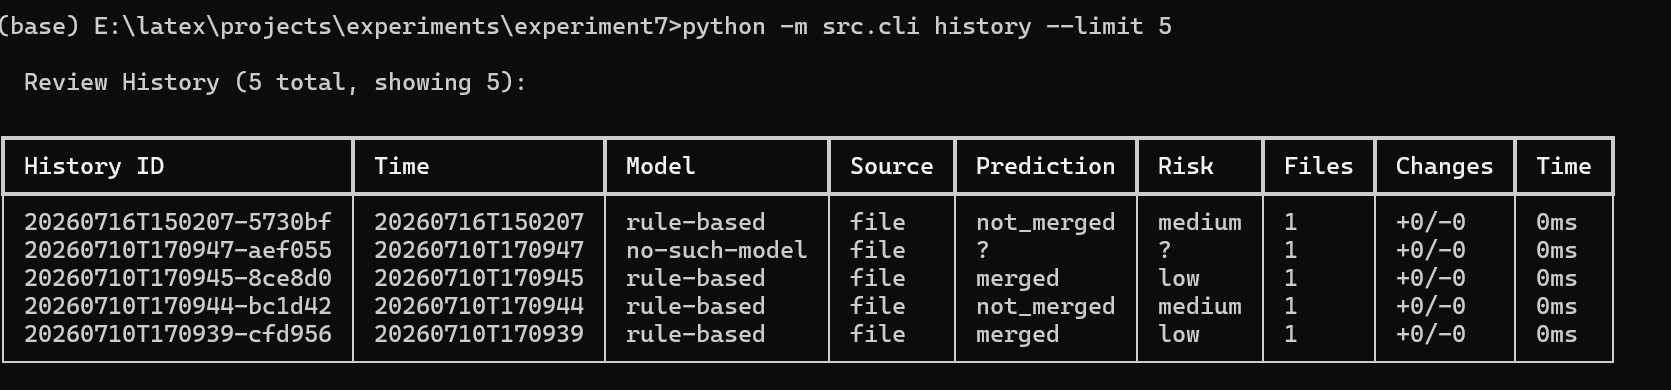
\includegraphics[width=0.95\textwidth]{../figures/05_history_list.png}\caption{审查历史列表}\end{figure}
\begin{figure}[htbp]\centering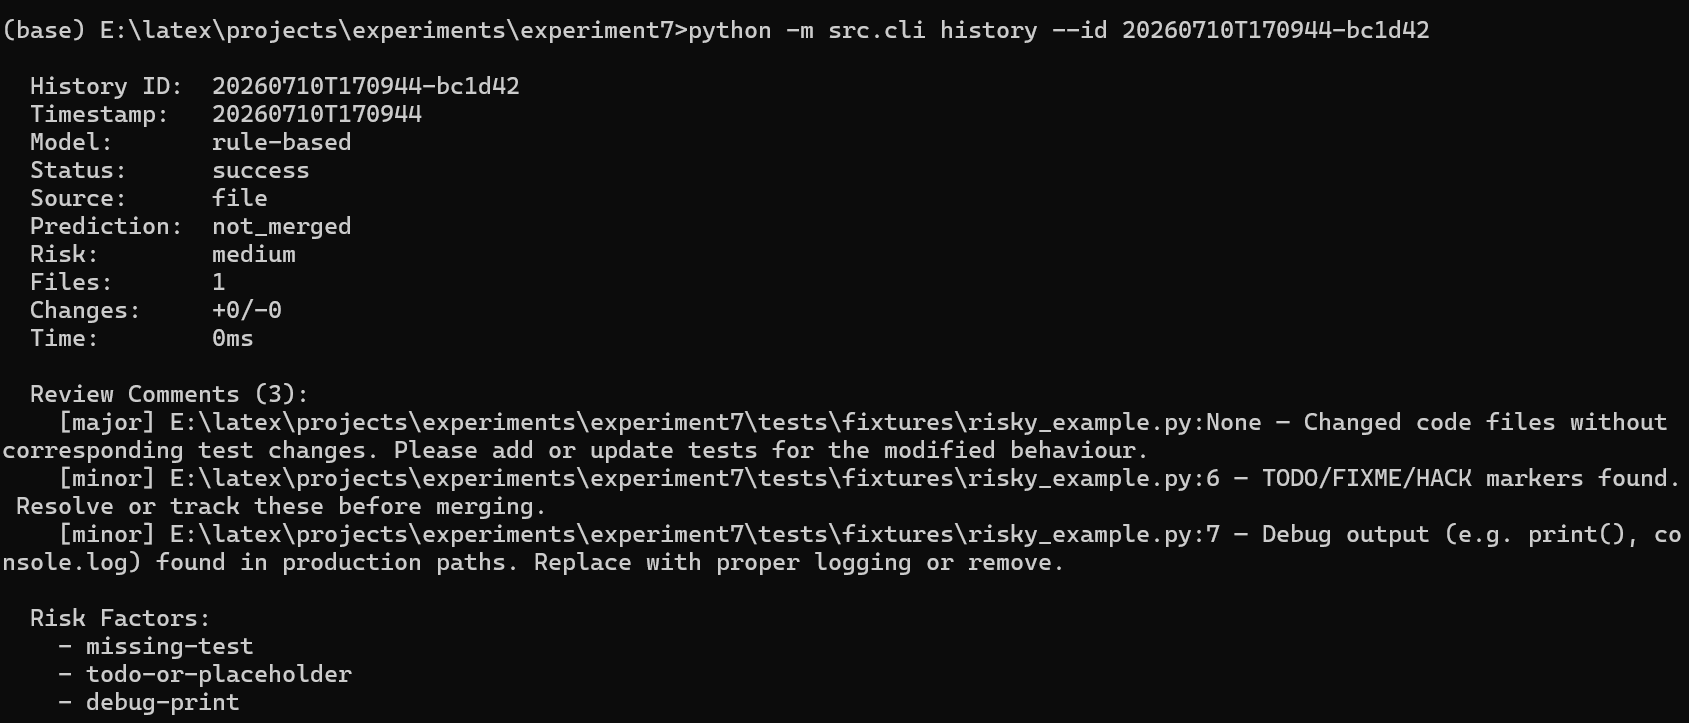
\includegraphics[width=0.95\textwidth]{../figures/06_history_detail.png}\caption{审查历史详情}\end{figure}
\begin{figure}[htbp]\centering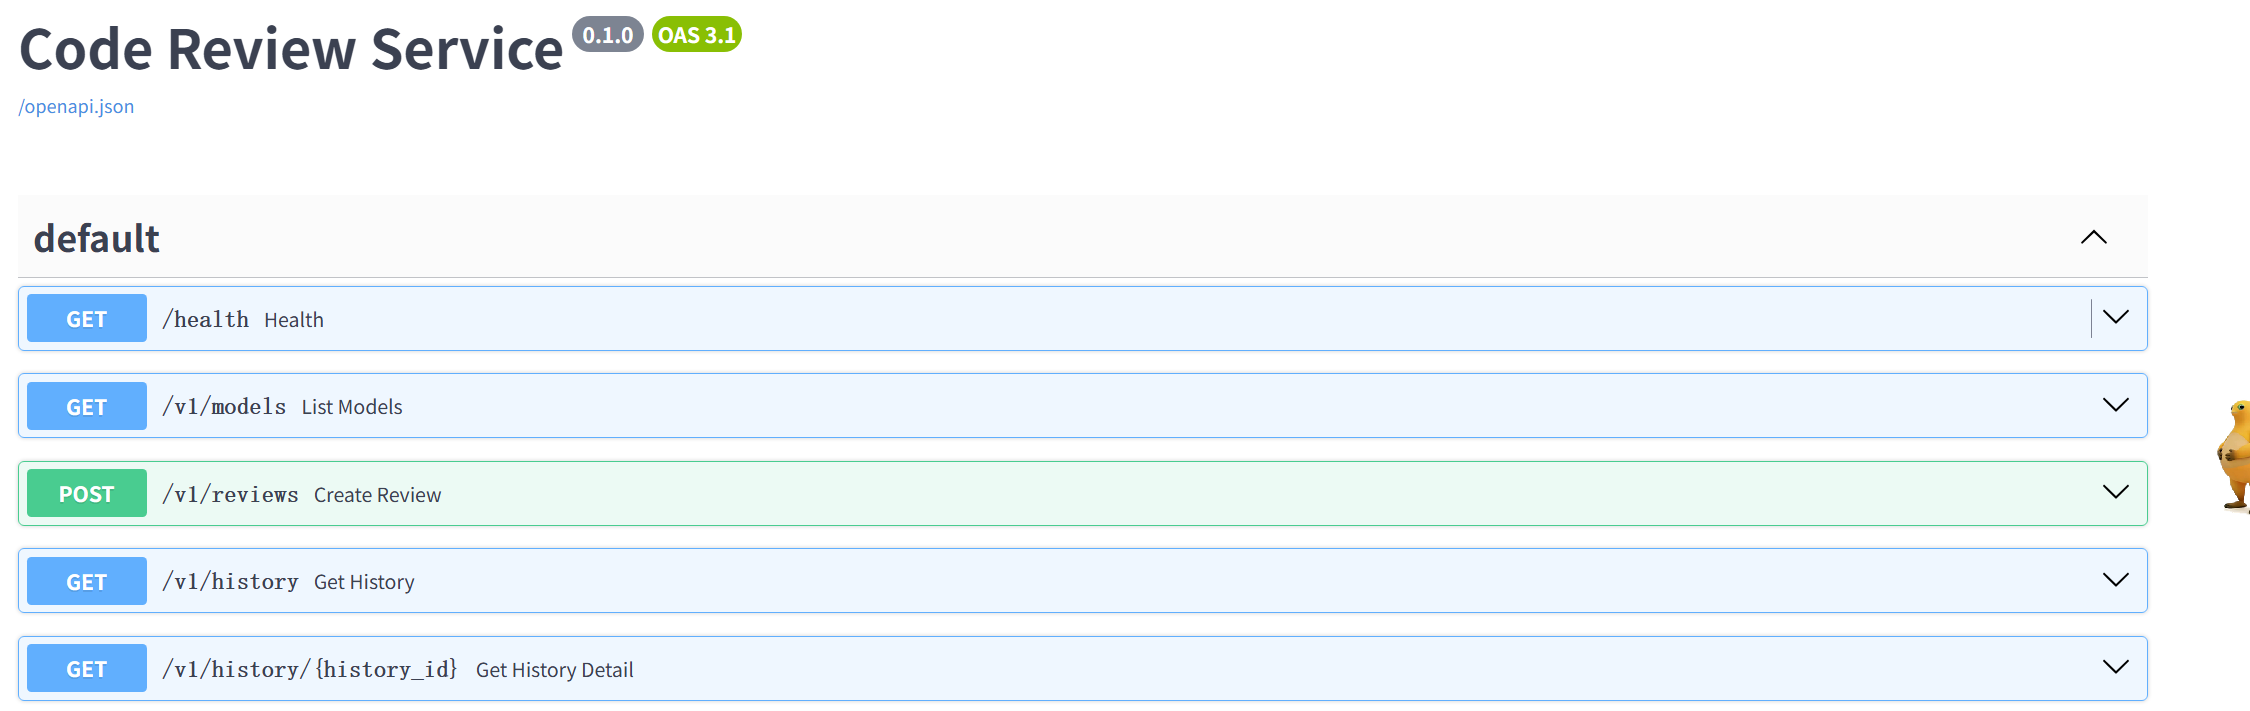
\includegraphics[width=0.95\textwidth]{../figures/07_api_docs.png}\caption{FastAPI自动生成的接口文档}\end{figure}
\begin{figure}[htbp]\centering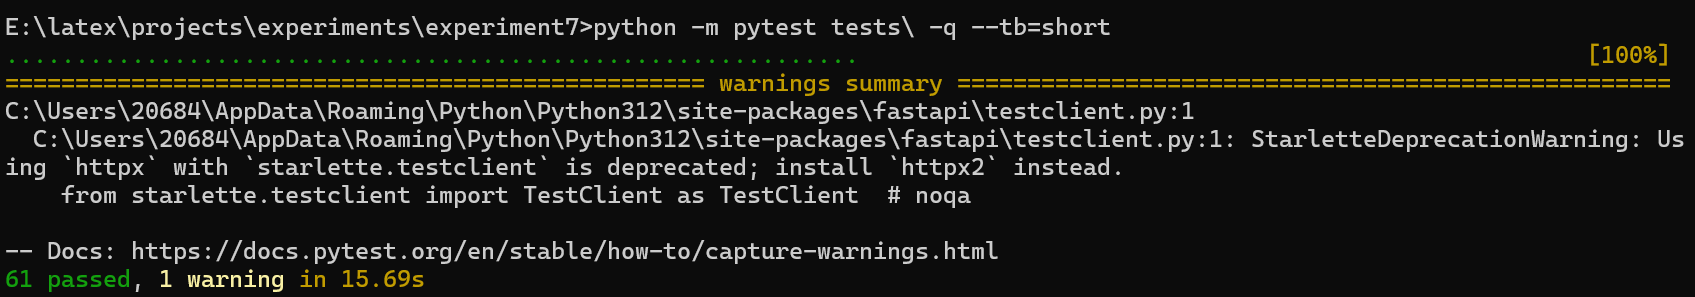
\includegraphics[width=0.95\textwidth]{../figures/08_tests.png}\caption{自动化测试结果}\end{figure}
\begin{figure}[htbp]\centering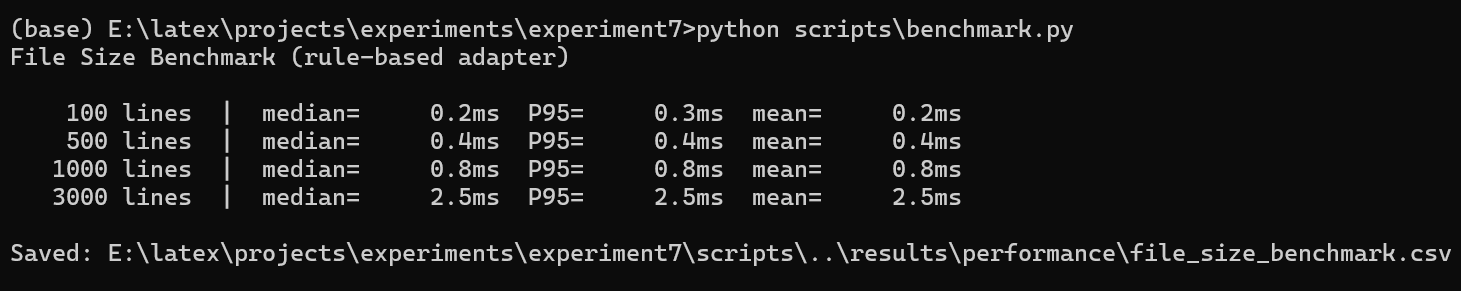
\includegraphics[width=0.95\textwidth]{../figures/09_benchmark.png}\caption{不同规模文件的规则模型性能测试}\end{figure}

% ═══════════════════════════════════════════════════════════════
\section{分析与局限}

\subsection{规则模型的局限}

\begin{itemize}
  \item 规则基于启发式模式匹配，不真正理解代码语义。
  \item 风险分数到合并概率的映射是线性的，不反映真实概率分布。
  \item 规则覆盖有限，无法检测复杂的逻辑缺陷、安全漏洞或性能问题。
  \item 行号定位依赖unified diff解析，在文件重命名或大范围重构时可能不准确。
\end{itemize}

\subsection{LLM适配的局限}

\begin{itemize}
  \item 依赖外部API，引入网络延迟和可用性风险。
  \item JSON输出格式不稳定，需要多层回退解析。
  \item 上下文窗口限制（24000字符截断），大PR可能丢失关键信息。
  \item API Key仅临时存在于运行会话，未持久化保存；服务重启后需重新配置，且密钥不能写入代码、截图或报告。
\end{itemize}

\subsection{ML适配的局限}

\begin{itemize}
  \item 原始61维模型仍不适用于CLI；部署版的45维特征集减少了PR元数据，指标不能与原始模型直接横向比较。
  \item 部署版仅支持Git diff；单独文件没有新增/删除语义，不适合输入ML分类器。
  \item 特征分布差异：训练数据为5个大型开源项目的历史PR，与本地任意文件/diff的统计分布可能显著不同。
\end{itemize}

\subsection{CLI相比IDE的交互不足}

\begin{itemize}
  \item 无法实现编辑器内代码高亮和行内标注。
  \item 无实时/自动触发机制（需手动执行命令）。
  \item 结果展示在终端，与代码编辑上下文分离。
  \item 缺少diff可视化、问题导航和快速修复等IDE功能。
\end{itemize}

% ═══════════════════════════════════════════════════════════════
\section{实验思考}

\subsection{为什么代码审查工具需要集成到IDE中？}

代码审查工具集成到IDE中可以缩短反馈周期——开发者在编写代码的同时即可获得审查意见，无需切换到终端或其他工具。IDE可以利用当前编辑器状态（打开的文件、未提交的diff、光标位置等）提供上下文感知的审查。本实验的CLI方案验证了服务边界和协议设计，IDE只需成为新的客户端——这也正是HTTP前后端分离架构的优势：替换前端不需要修改后端。

\subsection{前后端分离架构相比本地部署有哪些优势？}

\begin{itemize}
  \item \textbf{模型独立升级}：更新模型版本、切换模型类型不影响客户端。
  \item \textbf{客户端轻量}：CLI/IDE插件不依赖PyTorch、Transformers等重型框架。
  \item \textbf{统一协议}：所有客户端通过同一HTTP契约通信，便于测试和文档生成（OpenAPI）。
  \item \textbf{权限隔离}：API Key只在服务端配置，不暴露给每个客户端。
  \item \textbf{代价}：需要启动服务进程、引入网络延迟和版本兼容问题。
\end{itemize}

\subsection{如何提高插件的响应速度和用户体验？}

\begin{itemize}
  \item diff和代码内容截断，减少传输和推理开销。
  \item 内容SHA-256缓存，避免重复审查相同内容。
  \item 异步/后台调用，不阻塞编辑器。
  \item 离线规则模型快速反馈（本实验rule-based典型耗时<50ms）。
  \item LLM超时设置和可解释错误信息，避免无限等待。
  \item 清晰的进度指示和模型状态显示。
\end{itemize}

\subsection{插件部署过程中遇到了哪些工程问题？如何解决？}

\begin{enumerate}
  \item \textbf{Git状态差异}：clean工作区、未跟踪文件、二进制文件等边界情况需要专门的错误处理。解决：对每种情况分别检测并给出中文错误信息。
  \item \textbf{二进制/超大文件}：文件大小检查、null字节检测、编码异常捕获。解决：三层防护——文件大小上限、null字节检测、UTF-8解码异常处理。
  \item \textbf{行号映射}：unified diff到源文件行号的映射在复杂diff中可能不可靠。解决：新增文件使用新文件行号；无法可靠定位时设为null。
  \item \textbf{LLM JSON不稳定}：大语言模型的JSON输出偶尔包含尾部逗号、markdown包裹或多余文本。解决：5级回退JSON解析器（从实验六llm\_runner.py迁移）。
  \item \textbf{旧ML特征不匹配}：原始61维PR模型含本地不可得元数据。解决：保留原模型为incompatible，并以相同数据和划分重训练45维部署兼容模型。
  \item \textbf{历史隐私}：源代码默认写入历史会泄漏敏感信息。解决：默认不保存源代码，仅记录SHA-256摘要和统计量。
  \item \textbf{fcntl跨平台}：fcntl是Unix专有模块，Windows不可用。解决：使用os.replace（在Windows和Unix上均为原子操作）。
\end{enumerate}

\subsection{如果进一步完善该插件，还可以增加哪些功能？}

\begin{itemize}
  \item \textbf{VSCode Extension}：在已有HTTP协议上开发真正的VSCode插件，实现编辑器内代码高亮、行内标注和问题导航。
  \item \textbf{GitHub PR集成}：支持在线Pull Request代码审查，与GitHub Checks API集成。
  \item \textbf{增量审查}：仅审查diff变更部分，缓存未修改文件的审查结果。
  \item \textbf{模型版本评测}：建立评测基准，对比不同模型版本在相同输入上的表现。
  \item \textbf{自动修复建议}：结合代码转换工具生成具体的修复补丁。
  \item \textbf{团队策略配置}：允许项目配置自定义规则集、严重度阈值和审批策略。
  \item \textbf{多智能体协同}：集成多个审查Agent，从不同维度（安全、性能、风格、可维护性）并行审查。
\end{itemize}

% ═══════════════════════════════════════════════════════════════
\section{结论}

本实验完成了命令行智能代码审查工具的全部核心功能：

\begin{itemize}
  \item FastAPI服务可启动，\texttt{/health}和\texttt{/v1/models}可访问。
  \item CLI能审查文件、Git diff，并通过HTTP获得结构化结果。
  \item 离线rule-based模型完成Merge Prediction和评论生成，不依赖外网即可演示。
  \item 审查历史可保存、列出、查看；敏感代码正文默认不写入历史。
  \item 实验六LLM适配器已完成真实API调用，密钥仅通过临时环境变量提供且未持久化保存。
  \item 实验二原始模型的兼容性由特征契约JSON记录；45维部署兼容RF/SVM已完成重训练并成功接入Git diff审查。
  \item 61个自动化测试全部通过，覆盖schema、提取器、分析器、历史存储、API和部署版ML调用。
  \item 性能基准已实际执行，100至3000行文件的规则模型中位耗时为0.2至2.5ms。
  \item LaTeX报告如实记录各项状态，不伪造模型预测或性能数据。
\end{itemize}

\textbf{尚未实现的增强功能}：VSCode插件UI、watch监听模式、GitHub Actions annotation格式输出。这些可在同一HTTP协议上作为新增客户端实现。

经教师同意以CLI等价替代VSCode插件要求，本实验验证了智能代码审查工具从算法模型到可运行工程系统的完整流程，实现了指导书要求的各项核心功能。

\end{document}
